\def\mySecNum{9.3}
\mySection{\mySecNum~Comparing options with respect to style, maturity, and strike}
%-------------- start slide -------------------------------%{{{ 1
\begin{frame}[fragile,t]
	\frametitle{European versus American options}

	\begin{align*}
		C_{\text{Amer}}(S,K,T) & \ge C_{\text{Eur}}(S,K,T) \\[1em]
		P_{\text{Amer}}(S,K,T) & \ge P_{\text{Eur}}(S,K,T) \\
	\end{align*}
\end{frame}
%-------------- end slide -------------------------------%}}}
%-------------- start slide -------------------------------%{{{ 1
\begin{frame}[fragile,t]
	\frametitle{Maximum and minimum option prices}

	\begin{align*}
		S\ge C_{\text{Amer}}(S,K,T) \ge C_{\text{Eur}}(S,K,T) \ge \max\left(0, \text{PV}_{0,T}(F_{0,T})-\text{PV}_{0,T}(K)\right)
	\end{align*}
	\bigskip
	\bigskip

	\begin{align*}
		K \ge P_{\text{Amer}}(S,K,T) \ge P_{\text{Eur}}(S,K,T) \ge \max\left(0,\text{PV}(K)-\text{PV}_{0,T}(F_{0,T})\right)
	\end{align*}
\end{frame}
%-------------- end slide -------------------------------%}}}
%-------------- start slide -------------------------------%{{{ 1
\begin{frame}[fragile,t]
	\frametitle{Early exercise for American options}
	\begin{center}
		Calls on stocks \textcolor{magenta}{with no dividend}
		\bigskip

		No early exercise! \\

		\bigskip
		\mySeparateLine
		\bigskip

		\begin{align*}
			C_{\text{Ame}}(S_t,K,T-t) & \ge 			C_{\text{Eur}}(S_t,K,T-t) \\
																& =
			\underbrace{\textcolor{magenta}{S_t - K}}_{\text{Exercise value}} +
			\underbrace{\textcolor{cyan}{P_{Eur}(S_t,K,T-t)}}_{\text{Insurance against $S_T<K$}} +
			\underbrace{\textcolor{cyan}{K\left(1-e^{-r(T-t)}\right)}}_{\text{Time value of money on $K$}} \\
			& \ge
			\textcolor{magenta}{S_t - K}
		\end{align*}
	\end{center}
\end{frame}
%-------------- end slide -------------------------------%}}}
%-------------- start slide -------------------------------%{{{ 1
\begin{frame}[fragile,t]
\begin{center}
	Instead of $C(S_t,K,T-t) \ge S_t - K$ one can prove a stronger version:
	\bigskip
	\begin{equation*}
		\textcolor{magenta}{C(S_t,K,T-t) \ge S_t - Ke^{-r(T-t)}}
	\end{equation*}

	\bigskip
	\mySeparateLine
	\bigskip

	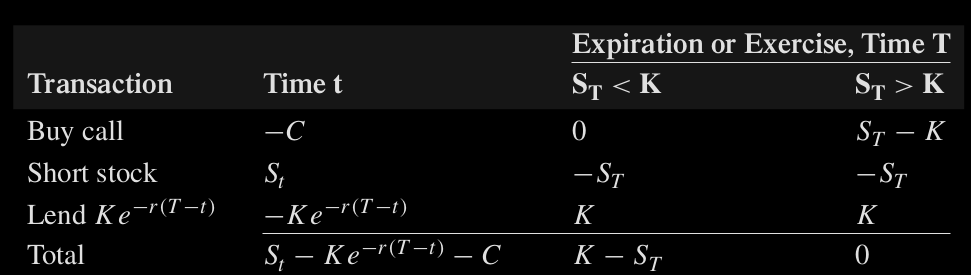
\includegraphics[scale=0.25]{figs/Table-9-4.png}

\end{center}
\end{frame}
%-------------- end slide -------------------------------%}}}
%-------------- start slide -------------------------------%{{{ 1
\begin{frame}[fragile,t]
	\frametitle{Early exercise for American options}
	\begin{center}
		Calls on stock \textcolor{cyan}{with dividends}
		\vfill

		\renewcommand{\arraystretch}{1.2}
		\begin{tabular}{|c|c|}
			\hline
			Interest beats dividends?                            & Early exercise? \\
			$K-\text{PV}_{t,T}(K) > \text{PV}_{t,T}(\text{Div})$ &                 \\ \hline
			\cmark                                               & \xmark          \\
			\xmark                                               & possibly        \\ \hline
		\end{tabular}

		\vfill

		When dividends do make early exercise rational, one should exercise \\
		at the last moment before the ex-dividend date.

	\end{center}
\end{frame}
%-------------- end slide -------------------------------%}}}
%-------------- start slide -------------------------------%{{{ 1
\begin{frame}[fragile,t]
	\begin{center}
		Early exercise for puts\\
		(no dividend case)
		\bigskip

		In order to receive interest, one may exercise early \\
		(think about the case when $S_T=0$)

		\bigskip

		\renewcommand{\arraystretch}{1.2}
		\begin{tabular}{cc}
			No early exercise & Early exercise \\ \hline
			$PV_{t,T}(K)$     & $K$            \\
		\end{tabular}

	\end{center}
\end{frame}
%-------------- end slide -------------------------------%}}}
%-------------- start slide -------------------------------%{{{ 1
\begin{frame}[fragile,t]
	\begin{center}
		Early exercise for puts\\
		(no dividend case)
		\bigskip


		No-exercise condition:
		\bigskip

		\begin{gather*}
			\textcolor{magenta}{P\left(S_t,K,T-t\right) > K -S_t} \\[1em]
			\Updownarrow                                          \\[1em]
			\textcolor{cyan}{C\left(S_t,K,T-t\right) > K - \text{PV}_{t,T}(K)}
		\end{gather*}

		\bigskip
		\mySeparateLine
		\bigskip

		\begin{equation*}
			P(S_t,K,T-t) = C(S_t,K,T-t) - S_t + \text{PV}_{t,T}(K)
		\end{equation*}
	\end{center}
\end{frame}
%-------------- end slide -------------------------------%}}}
%-------------- start slide -------------------------------%{{{ 1
\begin{frame}[fragile]
	\begin{center}
\renewcommand{\arraystretch}{1.2}
		\begin{tabular}{|c|cc|}
			\hline
                                    & calls                                     & puts                                  \\ \hline
			Receive                       & stock                                     & cash                                  \\
			Motivation for early exercise & \textcolor{magenta}{sufficient dividends} & \textcolor{cyan}{sufficient interest} \\ \hline
		\end{tabular}
		\bigskip
		\bigskip

		One can view interest as the dividend on cash. \\

		\bigskip
		Dividends are the sole reason to early-exercise an option.
	\end{center}
\end{frame}
%-------------- end slide -------------------------------%}}}
%-------------- start slide -------------------------------%{{{ 1
\begin{frame}[fragile]
	\frametitle{Time to expiration \\  -- the $K$ fixed}
	\begin{center}
		The longer the \textcolor{magenta}{more expensive}
		\bigskip

		\pause
		\begin{minipage}{0.7\textwidth}
			\begin{itemize}
				\item American call/put options
				\item European call option on stock with no dividend
					\begin{equation*}
						C_{Eur} = C_{Ame}
					\end{equation*}
			\end{itemize}
		\end{minipage}
	\end{center}

	\pause
	\mySeparateLine
	\bigskip
	\begin{center}
		The longer, might be \textcolor{cyan}{cheaper}
		\bigskip

		\pause
		\begin{minipage}{0.7\textwidth}
			\begin{itemize}
				\item European call option on stock with dividend
				\item European put option
			\end{itemize}
		\end{minipage}
	\end{center}
\end{frame}
%-------------- end slide -------------------------------%}}}
%-------------- start slide -------------------------------%{{{ 1
\begin{frame}[fragile]
	\frametitle{Time to expiration \\  -- $K_t=k e^{rt}$}

	\begin{mythm}
		When $K_t=e^{rt} K$, i.e., the strike grows at the interest rate, the premiums on European calls
		and puts on a non-dividend-paying stock increases with time to maturity.
	\end{mythm}
	\bigskip
	\pause
	\begin{myproof} We only prove the case for puts and leave the calls as exercise. \\
		Let $T>t$. In order to show that
	  \begin{align*}
		 	 P_{\text{Euro}}(S_T, K_T, T) > P_{\text{Euro}}(S_t, K_t, t),
		\end{align*}
		it suffices to find an arbitrage when
	  \begin{align*}
		 	 P_{\text{Euro}}(S_T, K_T, T) \le P_{\text{Euro}}(S_t, K_t, t).
		\end{align*}
	\end{myproof}
\end{frame}
%-------------- end slide -------------------------------%}}}
%-------------- start slide -------------------------------%{{{ 1
\begin{frame}[fragile,t]
	\begin{myproof}[ (continued)] \\
		\begin{center}
			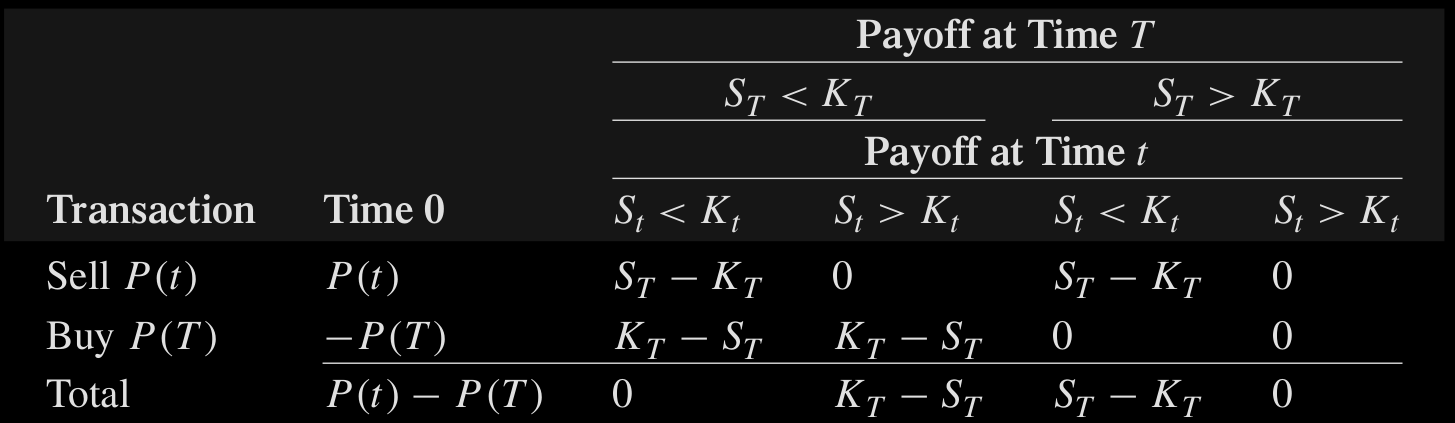
\includegraphics[scale=0.2]{figs/Table-9-5.png}
		\end{center}
		\bigskip

		For example, at time $t$, if $S_t<K_t$, one has to buy the stock. The payoff at time $t$ is
		\begin{equation*}
			S_t - K_t = S_t - K e^{rt}
		\end{equation*}
		One keeps this stock to time $T$, the stock price becomes  $S_T$, and the future value of
		$Ke^{rt}$ that one spent at time $t$ becomes  $Ke^{rt + r(T-t)}=Ke^{rT}$. Hence, the payoff of
		this strategy at time $T$ is
		\begin{equation*}
			S_T - Ke^{rT} = S_T - K_T.
		\end{equation*}
		\myEnd
	\end{myproof}
\end{frame}
%-------------- end slide -------------------------------%}}}
%-------------- start slide -------------------------------%{{{ 1
\begin{frame}[fragile,t]
	\frametitle{Different strike prices}
	\begin{center}
		$ K_1\le K_2 \le K_3$\\
		\bigskip

		\renewcommand{\arraystretch}{2.5}
		\begin{tabular}{|c|c|}
			\hline
			Relation                                                                         & Ideas in proof, arbitrage in          \\ \hline
			$C(K_1) \ge C(K_2)$                                                              & a call \textcolor{green}{bull} spread \\
			$P(K_1) \le P(K_2)$                                                              & a put \textcolor{red}{bear} spread    \\ \hline
			$C(K_1)-C(K_2) \le K_2-K_1$                                                      & a call \textcolor{red}{bear} spread   \\
			$P(K_2)-P(K_1) \le K_2-K_1$                                                      & a put \textcolor{green}{bull} spread  \\ \hline
			$ \displaystyle \frac{C(K_1)-C(K_2)}{K_2-K_1} \ge \frac{C(K_2)-C(K_3)}{K_3-K_2}$ & an asymmetric butterfly spread        \\
			$ \displaystyle \frac{P(K_2)-P(K_1)}{K_2-K_1} \le \frac{P(K_3)-P(K_2)}{K_3-K_2}$ & an asymmetric butterfly spread        \\ \hline
		\end{tabular}
	\end{center}
\end{frame}
%-------------- end slide -------------------------------%}}}
%-------------- start slide -------------------------------%{{{ 1
\begin{frame}[fragile,t]
\begin{center}
	Convexity revisited

	\begin{gather*}
		\frac{C(K_1)-C(K_2)}{K_2-K_1} \ge \frac{C(K_2)-C(K_3)}{K_3-K_2} \\[1em] \Updownarrow \\[1em]
		 C(K_2) \ge \lambda C(K_1) + (1-\lambda) C(K_3).
	\end{gather*}
	with
	\begin{align*}
		\lambda = \frac{K_3-K_2}{K_3-K_1}
	\end{align*}
\end{center}
\end{frame}
%-------------- end slide -------------------------------%}}}
%-------------- start slide -------------------------------%{{{ 1
\begin{frame}[fragile,t]
\begin{myexample}
	Suppose that
	\begin{center}
		\renewcommand{\arraystretch}{1.2}
		\begin{tabular}{ccc}
			Strike       & 50 & 55 \\
			Call Premium & 18 & 12 \\
		\end{tabular}
		\begin{enumerate}
			\item What no-arbitrage property is violated?
			\item What spread position would you use to effect arbitrage?
			\item Demonstrate that the spread position is an arbitrage.
		\end{enumerate}
	\end{center}
\end{myexample}
\pause
\bigskip
\begin{mysol}
	\textcolor{gray}{Check Example 9.4 on p. 283.} \myEnd
\end{mysol}
\end{frame}
%-------------- end slide -------------------------------%}}}
%-------------- start slide -------------------------------%{{{ 1
\begin{frame}[fragile,t]
\begin{myexample}
	Suppose that
	\begin{center}
		\renewcommand{\arraystretch}{1.2}
		\begin{tabular}{cccc}
			Strike       & 50 & 59  & 65 \\
			Call premium & 14 & 8.9 & 5  \\
		\end{tabular}
		\begin{enumerate}
			\item What no-arbitrage property is violated?
			\item What spread position would you use to effect arbitrage?
			\item Demonstrate that the spread position is an arbitrage.
		\end{enumerate}
	\end{center}
\end{myexample}
\pause
\bigskip
\begin{mysol}
	\textcolor{gray}{Check Example 9.5 on p. 284.} \myEnd
\end{mysol}
\end{frame}
%-------------- end slide -------------------------------%}}}
%-------------- start slide -------------------------------%{{{ 1
\begin{frame}[fragile,t]
\begin{myexample}
	Suppose that
	\begin{center}
		\renewcommand{\arraystretch}{1.2}
		\begin{tabular}{cccc}
			Strike      & 50 & 55 & 70 \\
			Put premium & 4  & 8  & 16 \\
		\end{tabular}
		\begin{enumerate}
			\item What no-arbitrage property is violated?
			\item What spread position would you use to effect arbitrage?
			\item Demonstrate that the spread position is an arbitrage.
		\end{enumerate}
	\end{center}
\end{myexample}
\pause
\bigskip
\begin{mysol}
	\textcolor{gray}{Check Example 9.6 on p. 284.} \myEnd
\end{mysol}
\end{frame}
%-------------- end slide -------------------------------%}}}

